\documentclass[UTF8,zihao=-4]{ctexart}
\usepackage[a4paper,top=2.0cm,bottom=2.0cm,left=2.2cm,right=2.2cm]{geometry}
\usepackage{amsmath,amssymb,booktabs,tabularx,array}
\usepackage{graphicx,float,caption}
\usepackage{xcolor,listings,tcolorbox}
\usepackage{fancyhdr,lastpage}
\usepackage[hidelinks]{hyperref}

\definecolor{navy}{HTML}{183B63}
\definecolor{blue}{HTML}{2B6EAE}
\definecolor{green}{HTML}{2F8F49}
\definecolor{orange}{HTML}{DF7615}
\definecolor{purple}{HTML}{7651B5}
\definecolor{soft}{HTML}{F3F7FB}
\definecolor{line}{HTML}{C9D4DF}
\definecolor{codebg}{HTML}{F6F8FA}
\definecolor{headergray}{HTML}{777777}

\hypersetup{
  pdftitle={系统开发工具基础 - 第1周实验报告},
  pdfauthor={朱元清},
  colorlinks=true,
  linkcolor=blue,
  urlcolor=blue
}

\pagestyle{fancy}
\fancyhf{}
\fancyhead[L]{\small\color{headergray}系统开发工具基础}
\fancyhead[R]{\small\color{headergray}第 1 周实验报告}
\fancyfoot[C]{\small\color{headergray}第 \thepage\ 页 / 共 \pageref{LastPage} 页}
\renewcommand{\headrulewidth}{0.5pt}
\renewcommand{\headrule}{\hbox to\headwidth{\color{line}\leaders\hrule height \headrulewidth\hfill}}

\lstdefinestyle{shell}{
  language=bash,
  basicstyle=\ttfamily\footnotesize,
  backgroundcolor=\color{codebg},
  frame=single,
  rulecolor=\color{line},
  breaklines=true,
  columns=fullflexible,
  keepspaces=true,
  showstringspaces=false,
  xleftmargin=0.3em,
  xrightmargin=0.3em,
  aboveskip=0.6em,
  belowskip=0.7em
}

\newtcolorbox{summarybox}[1]{
  colback=soft,
  colframe=blue,
  boxrule=0.7pt,
  arc=2mm,
  title={#1},
  fonttitle=\bfseries,
  coltitle=navy
}

\newcommand{\experimentbanner}[3]{
  \begin{tcolorbox}[
    colback=soft,
    colframe=navy,
    boxrule=1pt,
    arc=2mm,
    left=4mm,right=4mm,top=2.5mm,bottom=2.5mm]
    \begin{tabularx}{\textwidth}{>{\Large\bfseries\color{navy}}p{2.7cm}X}
      实验#1 & {\large\bfseries\color{navy}#2}\quad{\normalsize（#3）}
    \end{tabularx}
  \end{tcolorbox}
}

\newcommand{\practicebanner}[2]{
  \begin{tcolorbox}[
    colback=soft,
    colframe=navy,
    boxrule=1pt,
    arc=2mm,
    left=4mm,right=4mm,top=2.5mm,bottom=2.5mm]
    \begin{tabularx}{\textwidth}{>{\Large\bfseries\color{navy}}p{2.7cm}X}
      实例 #1 & {\large\bfseries\color{navy}#2}
    \end{tabularx}
  \end{tcolorbox}
}

\captionsetup{font=small,labelfont=bf,labelsep=quad}
\setlength{\parindent}{2em}
\setlength{\parskip}{0.25em}

\begin{document}

\thispagestyle{fancy}
\vspace*{0.7cm}
\begin{center}
  {\fontsize{28}{34}\selectfont\bfseries 系统开发工具基础}\\[0.35cm]
  {\fontsize{22}{28}\selectfont 第 1 周实验报告}\\[1.0cm]
  {\Large 姓名：朱元清\qquad 学号：25020007193}\\[0.6cm]
  {\Large 2026 年 8 月 24 日}
\end{center}

\vspace{0.7cm}
\begin{tcolorbox}[
  colback=soft,
  colframe=navy,
  boxrule=0.8pt,
  arc=2mm,
  left=5mm,right=5mm,top=4mm,bottom=4mm]
  \centering
  \normalsize
  本报告记录第 1 周四道实验题的执行命令与验证结果，内容覆盖 Shell 文件整理、
  管道文本统计、Git 合并冲突处理和 LaTeX 文档构建。
\end{tcolorbox}

\vspace{0.65cm}
\begin{table}[H]
  \centering
  \caption{第 1 周实验完成情况}
  \renewcommand{\arraystretch}{1.35}
  \begin{tabularx}{0.92\textwidth}{cX>{\raggedright\arraybackslash}p{4.4cm}c}
    \toprule
    实验 & 主题 & 关键工具 & 状态 \\
    \midrule
    1 & 含空格文件名的批量整理 & Shell、find、chmod & \textcolor{blue}{\checkmark\ 完成} \\
    2 & 随机访问日志统计 & awk、sort、head & \textcolor{green}{\checkmark\ 完成} \\
    3 & 制造并解决一次合并冲突 & Git、merge & \textcolor{orange}{\checkmark\ 完成} \\
    4 & 修复并构建一页技术说明 & LaTeX、交叉引用 & \textcolor{purple}{\checkmark\ 完成} \\
    \bottomrule
  \end{tabularx}
\end{table}

\vfill
\experimentbanner{一}{含空格文件名的批量整理}{Shell 基础与文件系统}
\newpage

\subsection*{执行命令}
\begin{lstlisting}[style=shell]
mkdir q01 && cd q01
mkdir -p input/{docs,tmp}
printf 'alpha\nbeta\n' > "input/docs/notes one.txt"
printf 'hidden\n' > input/docs/.secret.txt
: > input/tmp/empty.txt
printf 'start\nend\n' > input/run.log

pwd
ls -la input

STUDENT_ID=25020007193
mkdir -p "work/$STUDENT_ID"
find input -type f -name '*.txt' \
  -exec cp --parents {} "work/$STUDENT_ID/" \;
find "work/$STUDENT_ID" -type d -exec chmod 750 {} +
find "work/$STUDENT_ID" -type f -exec chmod 640 {} +
find "work/$STUDENT_ID/input" -type f -name '*.txt' \
  -printf '%P\t%s\n' | sort > inventory.txt
cat inventory.txt
\end{lstlisting}

\begin{figure}[H]
  \centering
  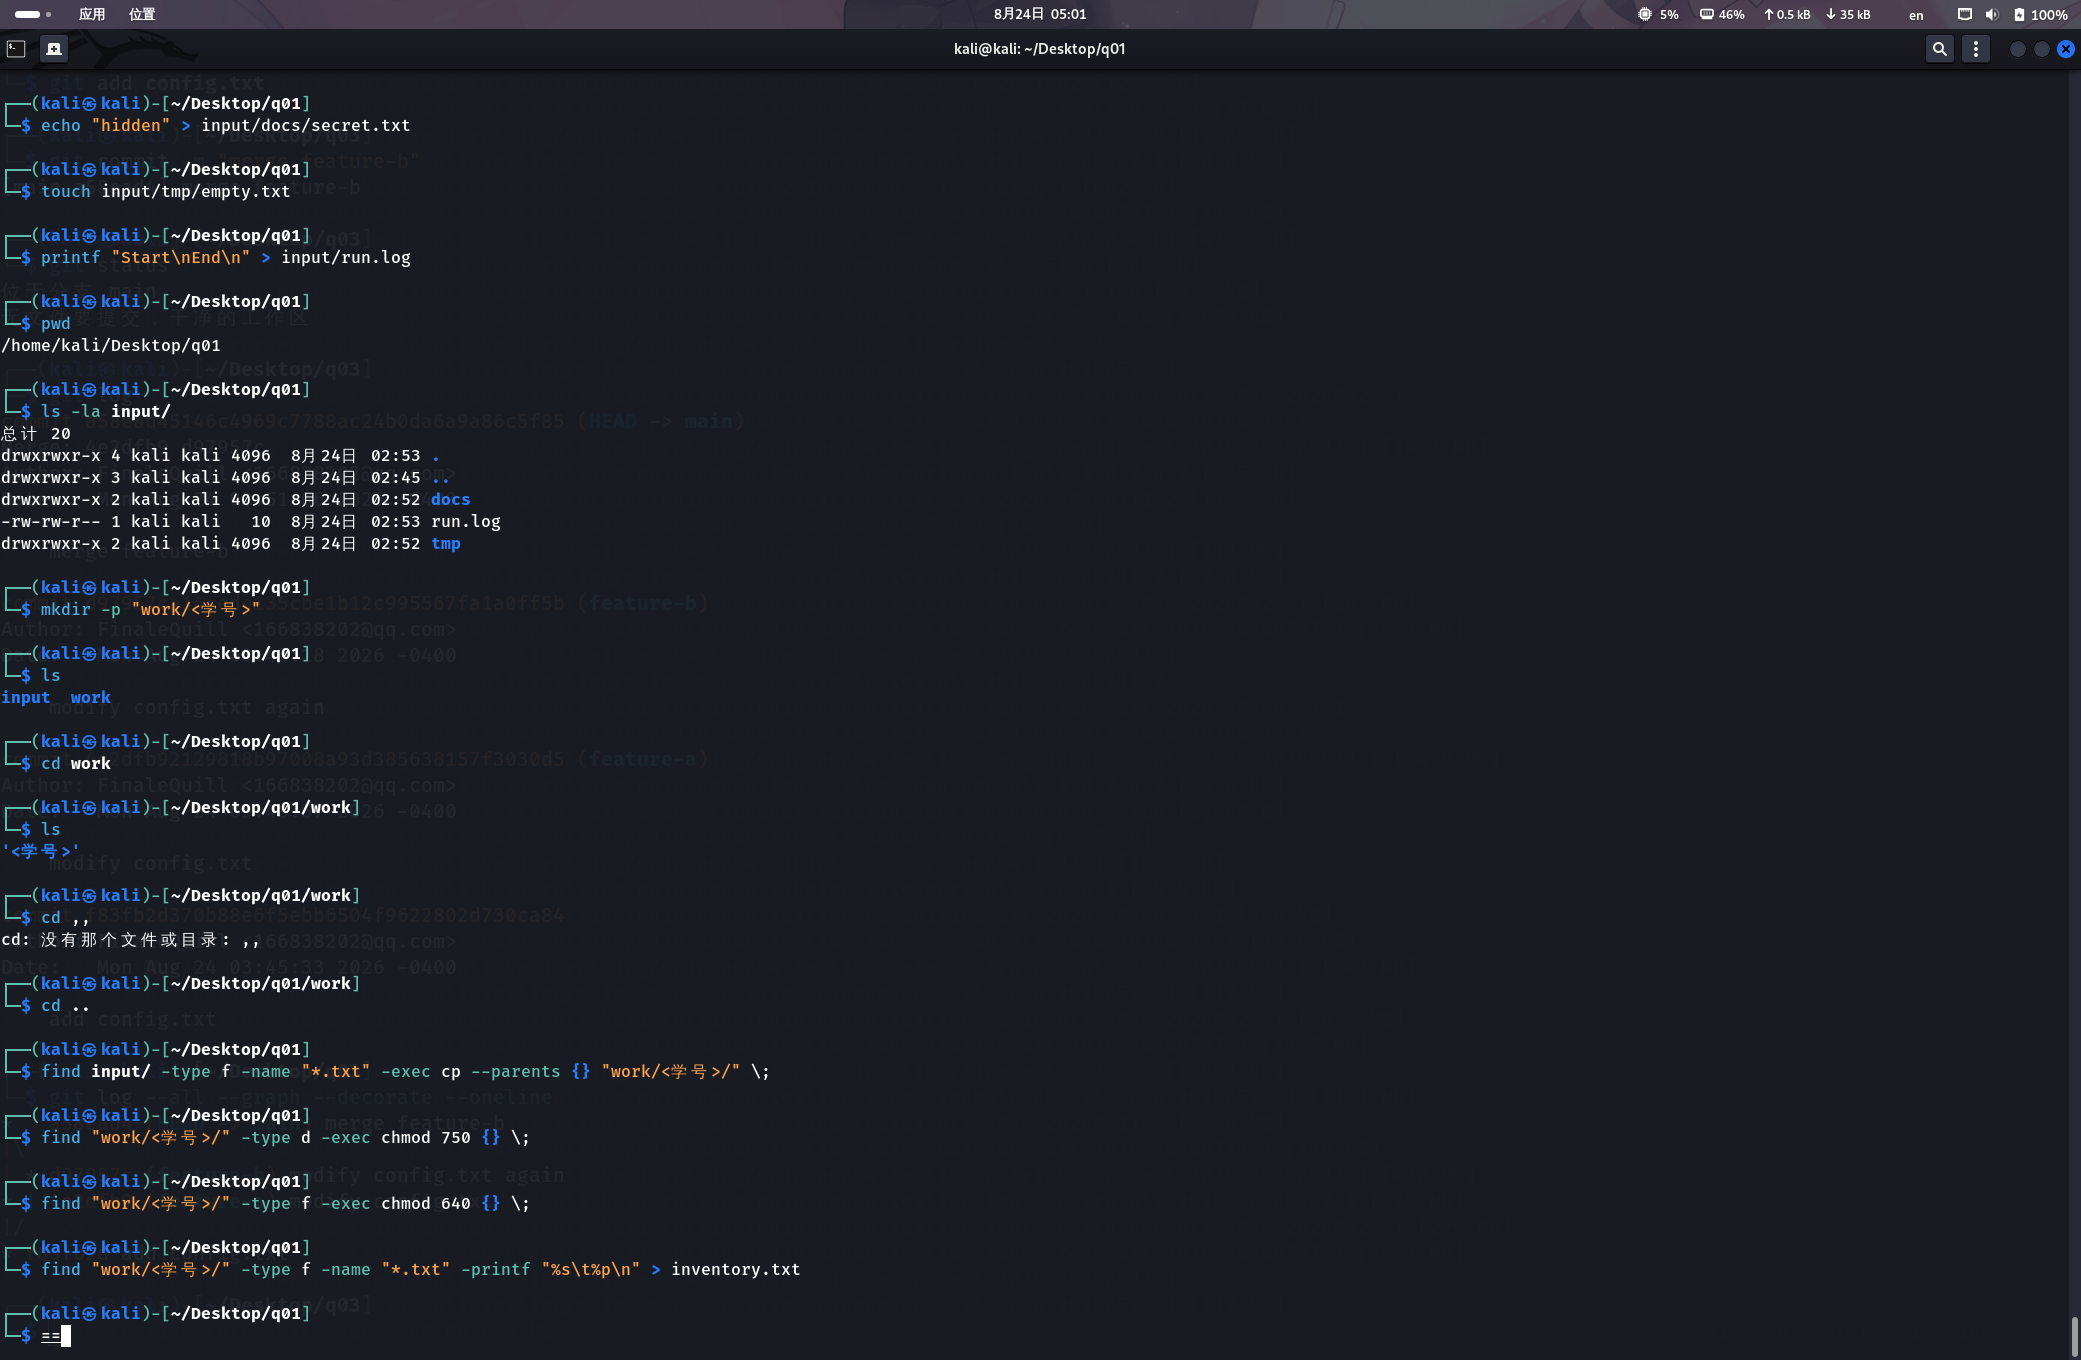
\includegraphics[width=.88\textwidth,height=.46\textheight,keepaspectratio]{assets/q01-run.png}
  \caption{实验一运行结果}
\end{figure}

\begin{summarybox}{结果说明}
完成目录和测试文件创建，复制后的目录结构得到保留；目录权限为 750，普通文件权限
为 640，\texttt{inventory.txt} 列出了各文本文件的相对路径和字节数。
\end{summarybox}

\clearpage
\experimentbanner{二}{随机访问日志统计}{Shell 管道与文本处理}

\subsection*{执行命令}
\begin{lstlisting}[style=shell]
mkdir q02 && cd q02
cat > access.csv <<'EOF'
timestamp,user,path,status,latency_ms
09:00:01,alice,/api/users,200,120
09:00:02,bob,/api/orders,500,310
09:00:03,alice,/api/users,503,180
09:00:04,carol,/login,500,90
09:00:05,bob,/api/orders,502,260
09:00:06,dave,/health,200,20
09:00:07,alice,/api/orders,500,420
09:00:08,carol,/api/users,500,150
EOF

cat > analyze.sh <<'EOF'
#!/bin/bash
if [ "$#" -ne 1 ]; then
    echo "Usage: $0 <csv_file>" >&2
    exit 1
fi
csv_file="$1"
if [ ! -f "$csv_file" ]; then
    echo "Error: File '$csv_file' not found" >&2
    exit 1
fi

echo "Top 2 paths with most 5xx errors:"
awk -F, 'NR>1 && $4>=500 && $4<600 {count[$3]++}
          END {for (path in count) printf "%s\t%d\n", path, count[path]}' \
    "$csv_file" | sort -k2,2nr -k1,1 | head -n 2

avg=$(awk -F, 'NR>1 {sum += $5; n++}
               END {if(n>0) printf "%.2f", sum/n; else print "0.00"}' \
               "$csv_file")
echo "Average latency: $avg"
EOF

chmod +x analyze.sh
./analyze.sh access.csv
./analyze.sh nothing.csv
echo $?
\end{lstlisting}

\begin{figure}[H]
  \centering
  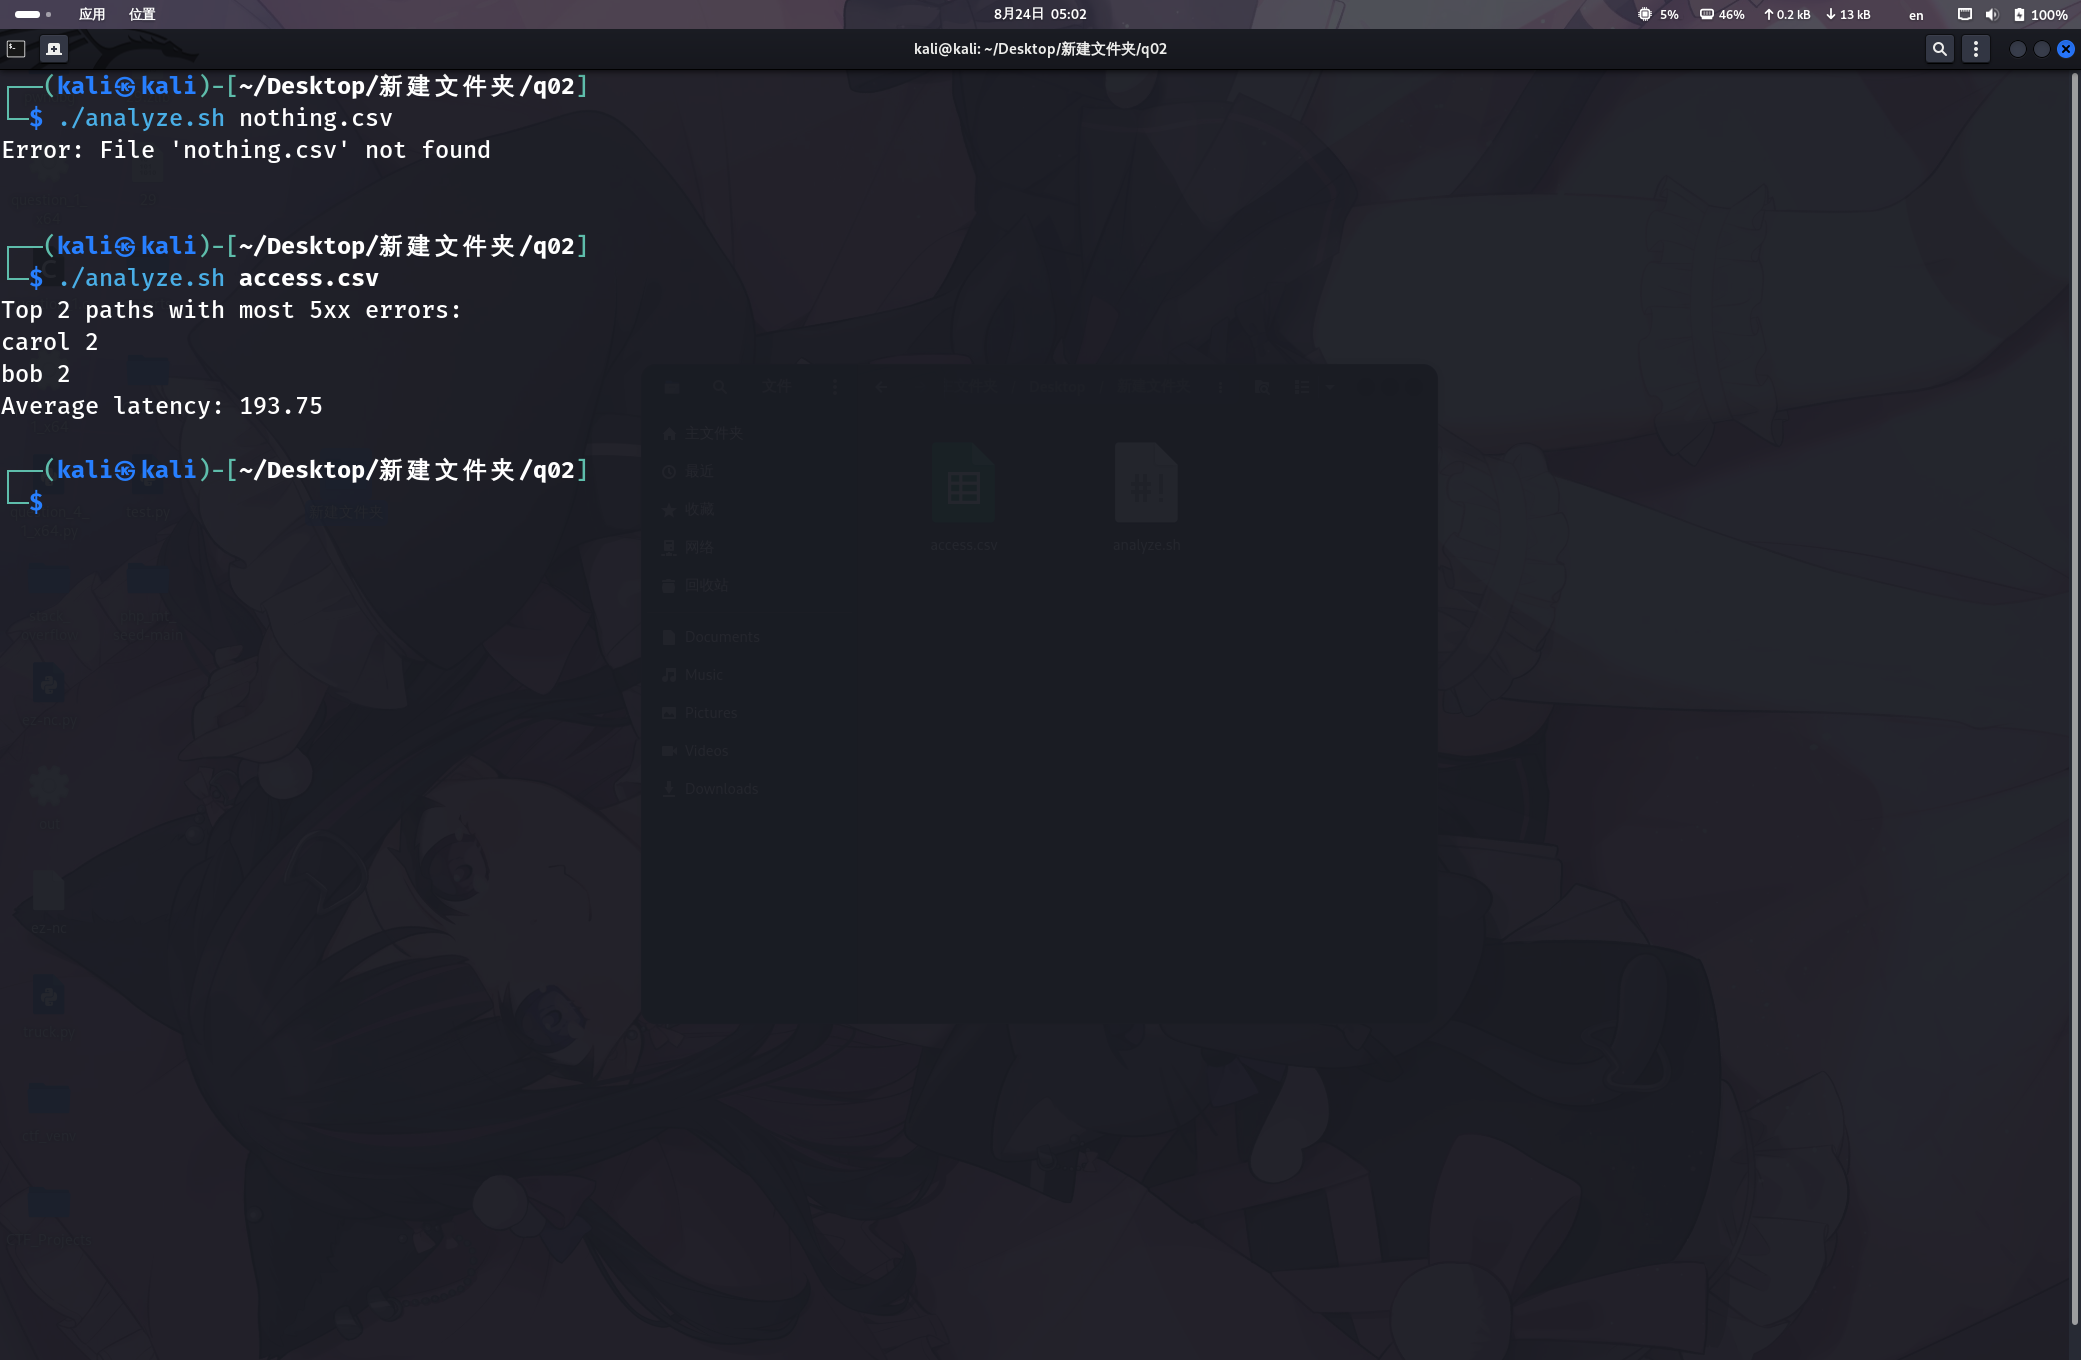
\includegraphics[width=\textwidth,height=.52\textheight,keepaspectratio]{assets/q02-run.png}
  \caption{实验二运行结果}
\end{figure}

\begin{summarybox}{结果说明}
脚本通过管道完成 5xx 路径计数和排序，并输出前 2 项；全部数据行的平均延迟为
\texttt{193.75 ms}。文件不存在时，错误信息写入 stderr，并返回非零退出码。
\end{summarybox}

\clearpage
\experimentbanner{三}{制造并解决一次合并冲突}{Version Control and Git}

\subsection*{执行命令}
\begin{lstlisting}[style=shell]
mkdir q03 && cd q03
git init -b main
printf 'mode=normal\n' > config.txt
git add config.txt
git commit -m 'add config.txt'
BASE=$(git rev-parse HEAD)

git switch -c feature-a
printf 'mode=safe\n' > config.txt
git add config.txt
git commit -m 'modify config.txt'

git switch -c feature-b "$BASE"
printf 'mode=fast\n' > config.txt
git add config.txt
git commit -m 'modify config.txt again'

git switch main
git merge feature-a
git merge feature-b
printf 'mode=safe\nnote=reviewed\n' > config.txt
git add config.txt
git commit -m 'merge feature-b'

git status
git log --all --graph --decorate --oneline
\end{lstlisting}

\begin{figure}[H]
  \centering
  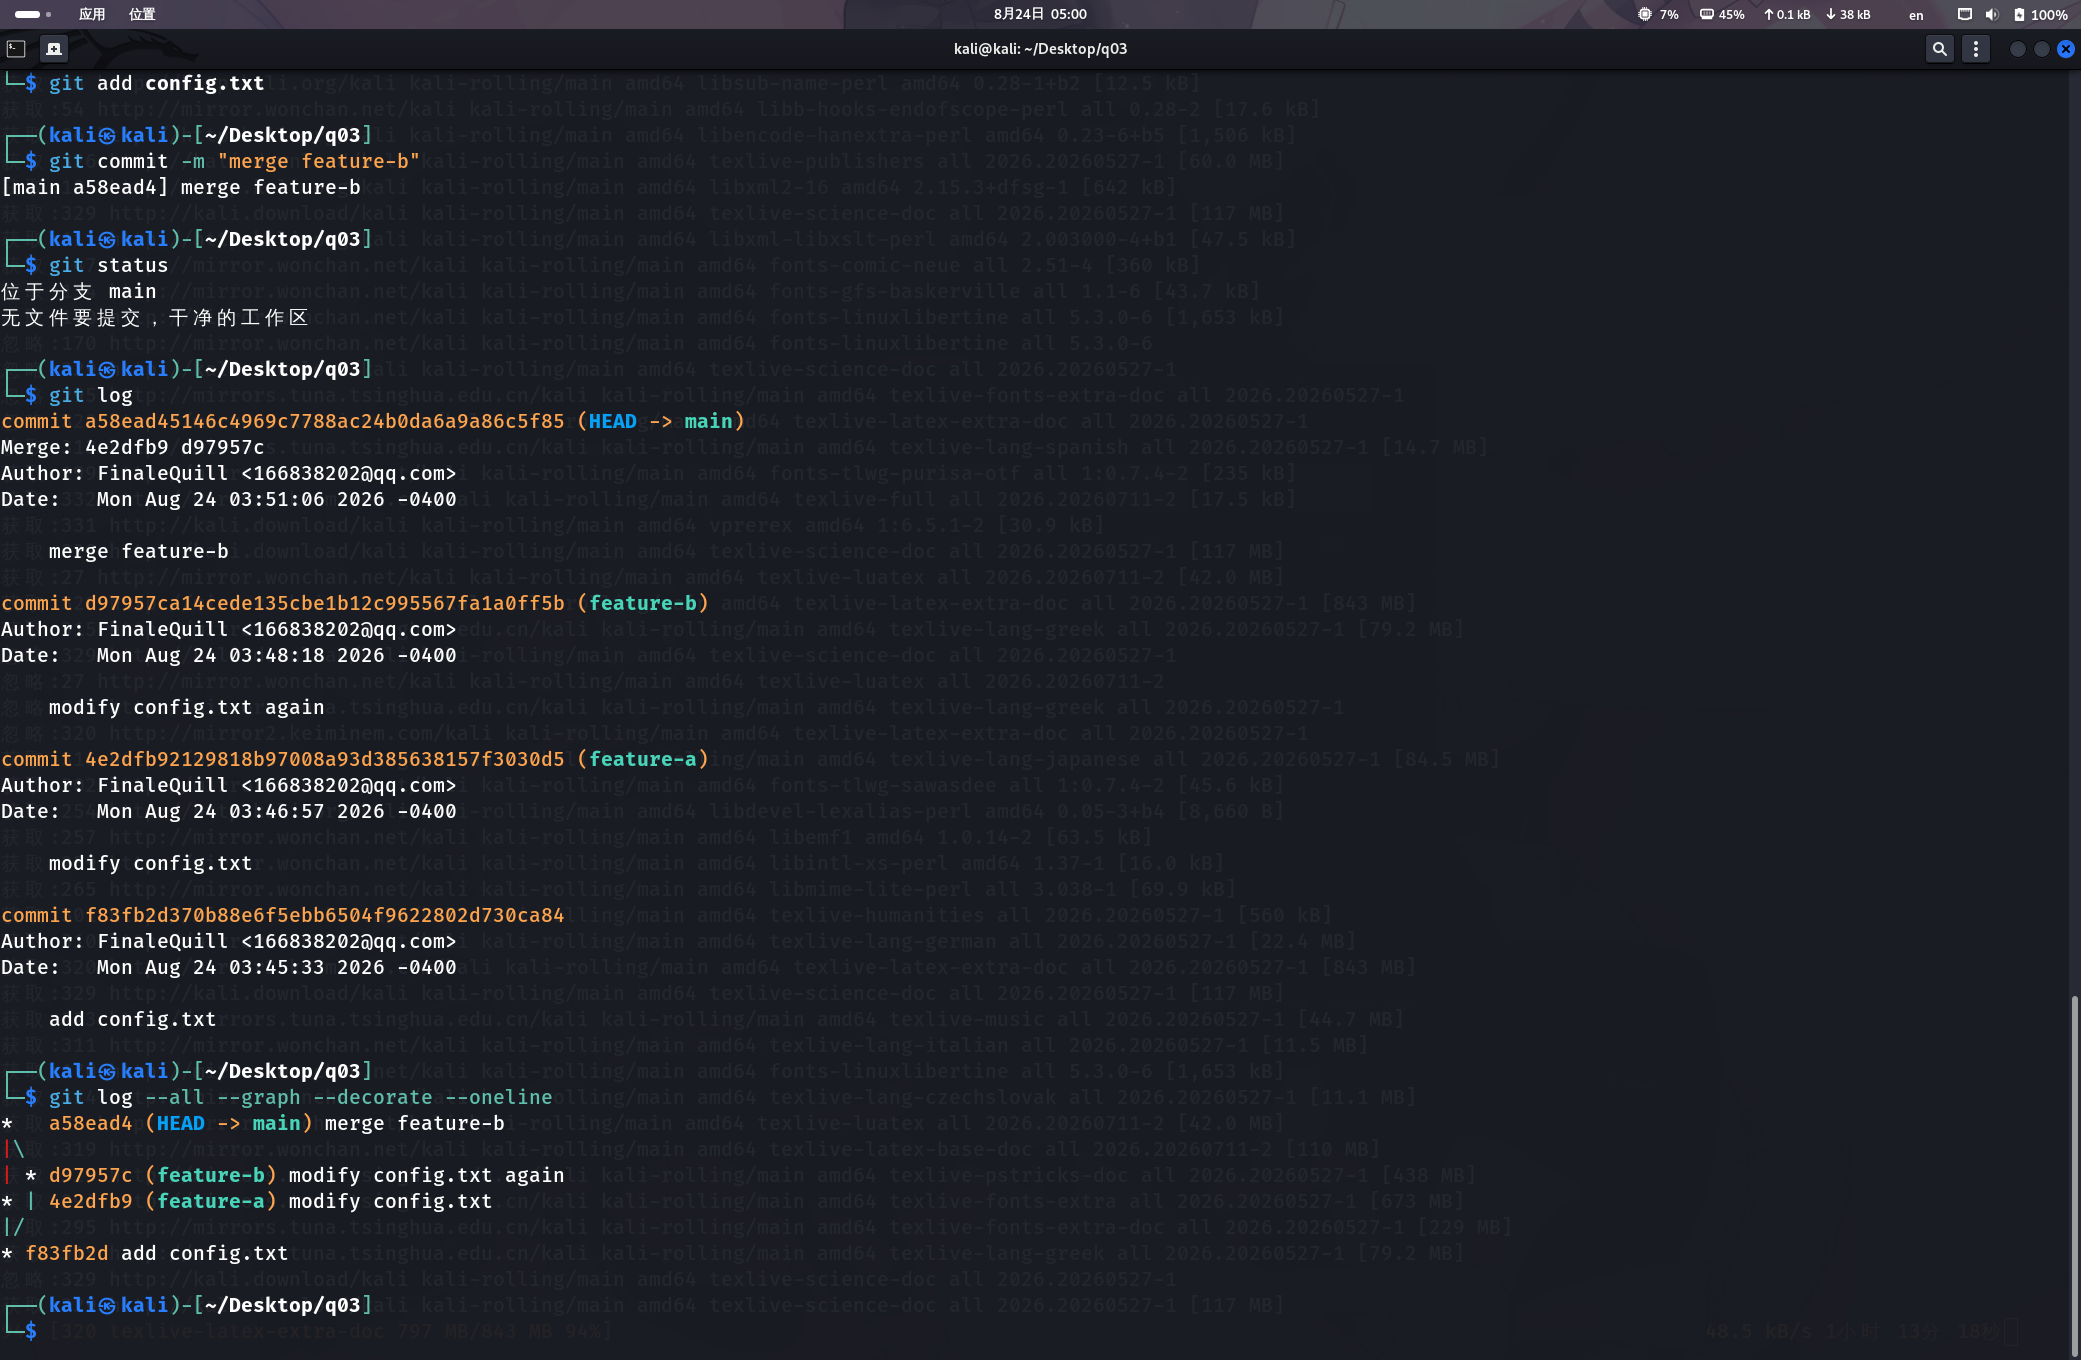
\includegraphics[width=\textwidth,height=.55\textheight,keepaspectratio]{assets/q03-run.png}
  \caption{实验三运行结果}
\end{figure}

\begin{summarybox}{结果说明}
两个特性分支对同一配置项写入不同值并产生合并冲突。冲突解决后，
\texttt{config.txt} 保留 \texttt{mode=safe} 和 \texttt{note=reviewed}，
工作区状态干净，提交图完整显示分支与合并过程。
\end{summarybox}

\clearpage
\experimentbanner{四}{修复并构建一页技术说明}{LaTeX 文档编辑}

\subsection*{执行命令}
\begin{lstlisting}[style=shell]
mkdir q04 && cd q04
cat > report.tex <<'EOF'
\documentclass[11pt]{article}
\usepackage[a4paper,margin=2.4cm]{geometry}
\usepackage{amsmath}
\usepackage{booktabs}
\usepackage{xcolor}
\usepackage[hidelinks]{hyperref}

\definecolor{accent}{HTML}{1F5A94}
\setlength{\parindent}{0pt}
\setlength{\parskip}{0.65em}

\begin{document}
\title{\textcolor{accent}{Tool Report}}
\author{Zhu Yuanqing -- 25020007193}
\date{August 24, 2026}
\maketitle

\section{Result}
For a data set containing $n$ latency measurements $t_i$, the arithmetic
mean is defined by Equation~\eqref{eq:mean-latency}.
\begin{equation}
  \bar{t}=\frac{1}{n}\sum_{i=1}^{n} t_i
  \label{eq:mean-latency}
\end{equation}
The build check in Table~\ref{tab:build-check} records the two essential
parts of this one-page technical note.

\begin{table}[htbp]
  \centering
  \caption{Build check}
  \label{tab:build-check}
  \begin{tabular}{cc}
    \toprule
    Item & Status \\
    Formula reference & Passed \\
    \bottomrule
  \end{tabular}
\end{table}
\end{document}
EOF

tectonic report.tex
\end{lstlisting}

\begin{figure}[H]
  \centering
  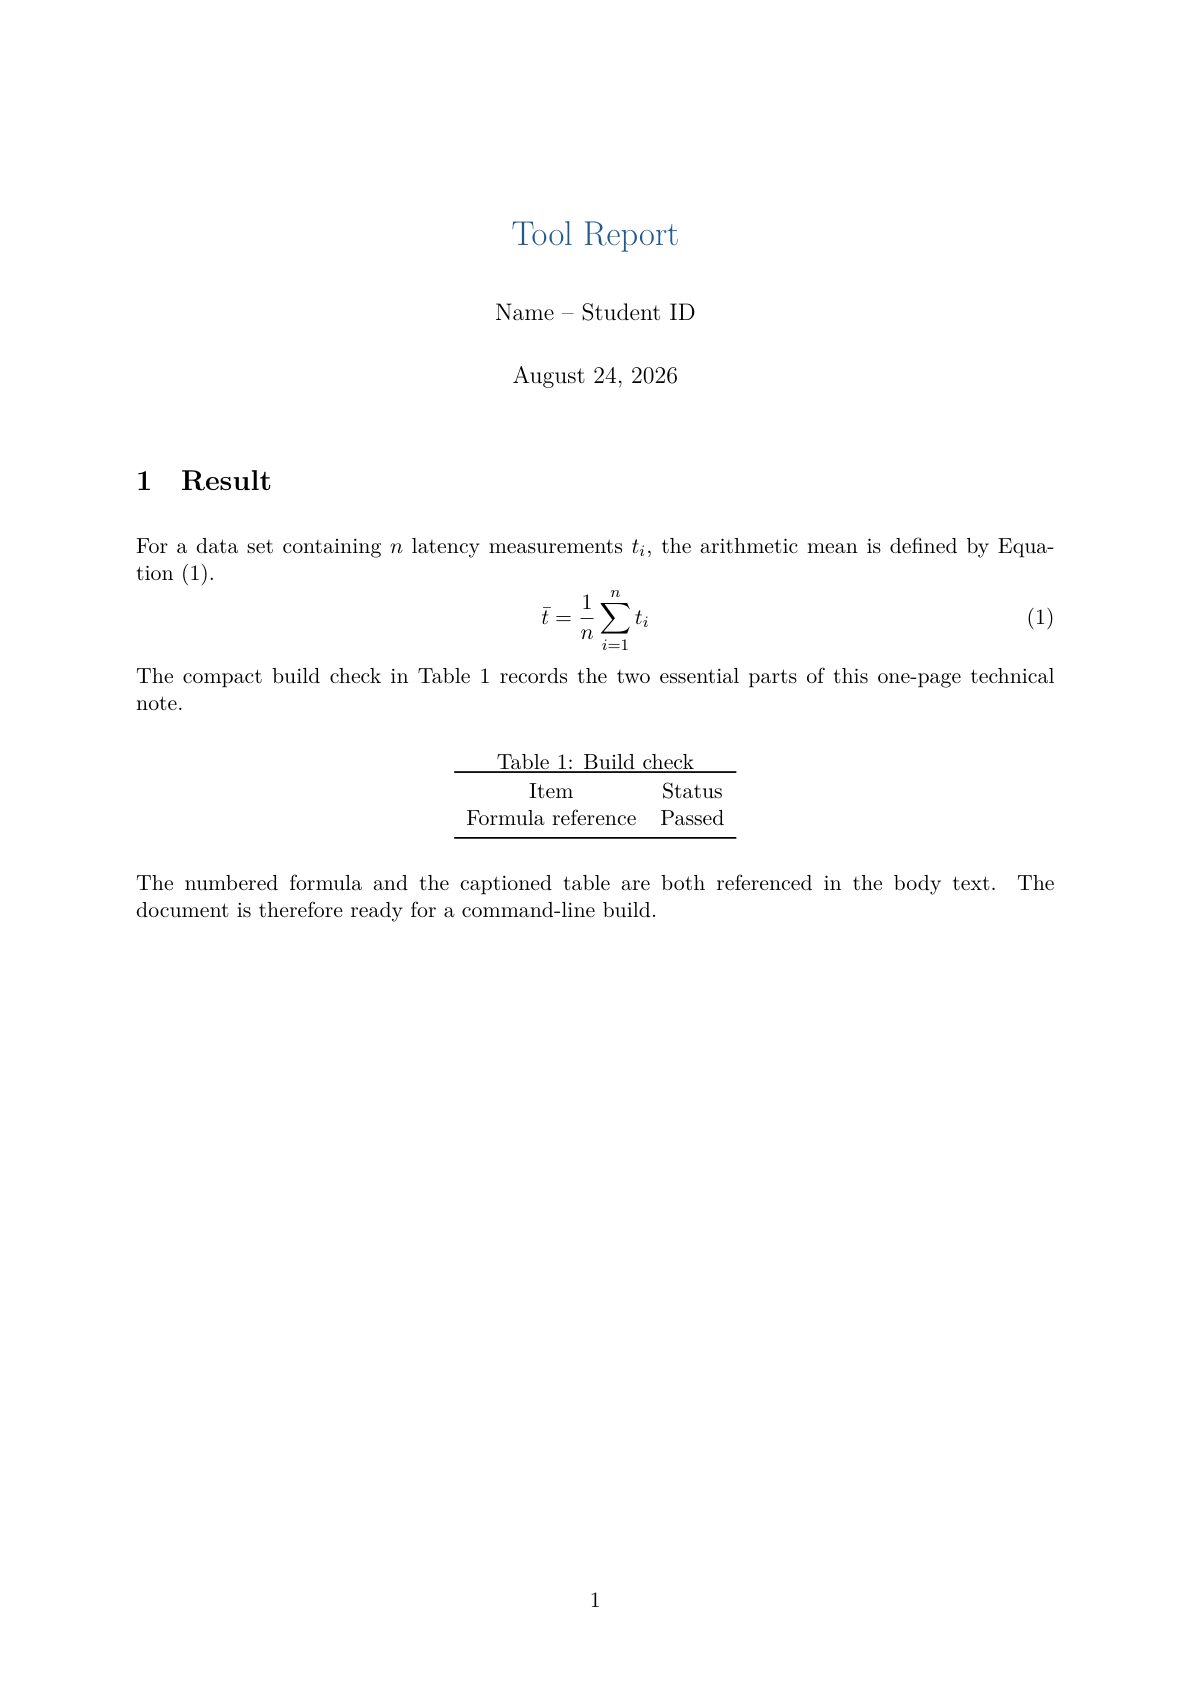
\includegraphics[width=.82\textwidth,height=.50\textheight,keepaspectratio,
    trim=0 260 0 300,clip]{assets/q04-output.png}
  \caption{实验四构建结果}
\end{figure}

\begin{summarybox}{结果说明}
命令行构建生成 \texttt{report.pdf}。编号公式和 2 行 2 列表格均设置了 label，
正文引用显示实际编号，PDF 可以正常打开。
\end{summarybox}

\clearpage
\vspace*{1.2cm}
\begin{center}
  {\fontsize{26}{32}\selectfont\bfseries 课后练习}\\[0.35cm]
  {\Large Shell 命令实例（选做 10 题）}
\end{center}

\vspace{0.9cm}
\begin{table}[H]
  \centering
  \caption{课后练习选题}
  \renewcommand{\arraystretch}{1.35}
  \begin{tabularx}{0.92\textwidth}{cX>{\raggedright\arraybackslash}p{5.2cm}}
    \toprule
    编号 & 实例内容 & 关键命令 \\
    \midrule
    1  & 确认 Unix Shell 环境 & \texttt{echo}、\texttt{bash} \\
    2  & 读取 \texttt{ls -l} 权限字段 & \texttt{ls -l} \\
    3  & 测试 Shell glob 模式 & \texttt{*}、\texttt{?}、花括号展开 \\
    4  & 比较三种引号 & 单引号、双引号、ANSI-C 引号 \\
    5  & 重定向标准输出与错误 & \texttt{>}、\texttt{2>}、\texttt{2>\&1} \\
    6  & 退出状态与条件执行 & \texttt{\$?}、\texttt{\&\&}、\texttt{||} \\
    7  & 验证 \texttt{cd} 是内建命令 & \texttt{type}、子 Shell \\
    8  & 用脚本检查文件是否存在 & \texttt{test -f} \\
    10 & 使用 \texttt{set -x} 跟踪命令 & \texttt{set -x} \\
    11 & 生成带日期的备份文件名 & \texttt{\$(date ...)} \\
    \bottomrule
  \end{tabularx}
\end{table}

\vfill
\practicebanner{1}{确认 Unix Shell 环境}

\clearpage
\subsection*{执行命令}
\begin{lstlisting}[style=shell]
echo "$SHELL"
bash --version | head -n 1
\end{lstlisting}

\begin{figure}[H]
  \centering
  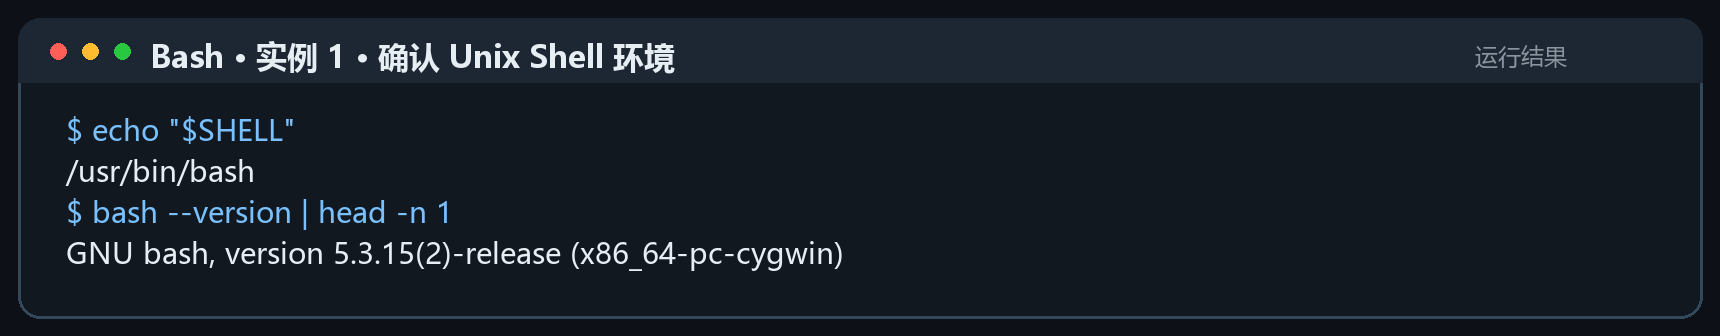
\includegraphics[width=.94\textwidth,height=.50\textheight,keepaspectratio]{assets/practice-ex01.png}
  \caption{实例 1 运行结果}
\end{figure}

\begin{summarybox}{结果说明}
Shell 路径为 \texttt{/usr/bin/bash}，版本信息由 Bash 正常输出，当前环境满足 Unix 风格 Shell 的使用要求。
\end{summarybox}

\clearpage
\practicebanner{2}{读取 \texttt{ls -l} 权限字段}

\subsection*{执行命令}
\begin{lstlisting}[style=shell]
ls -l /
ls -ld / /tmp /usr/bin/bash
\end{lstlisting}

\begin{figure}[H]
  \centering
  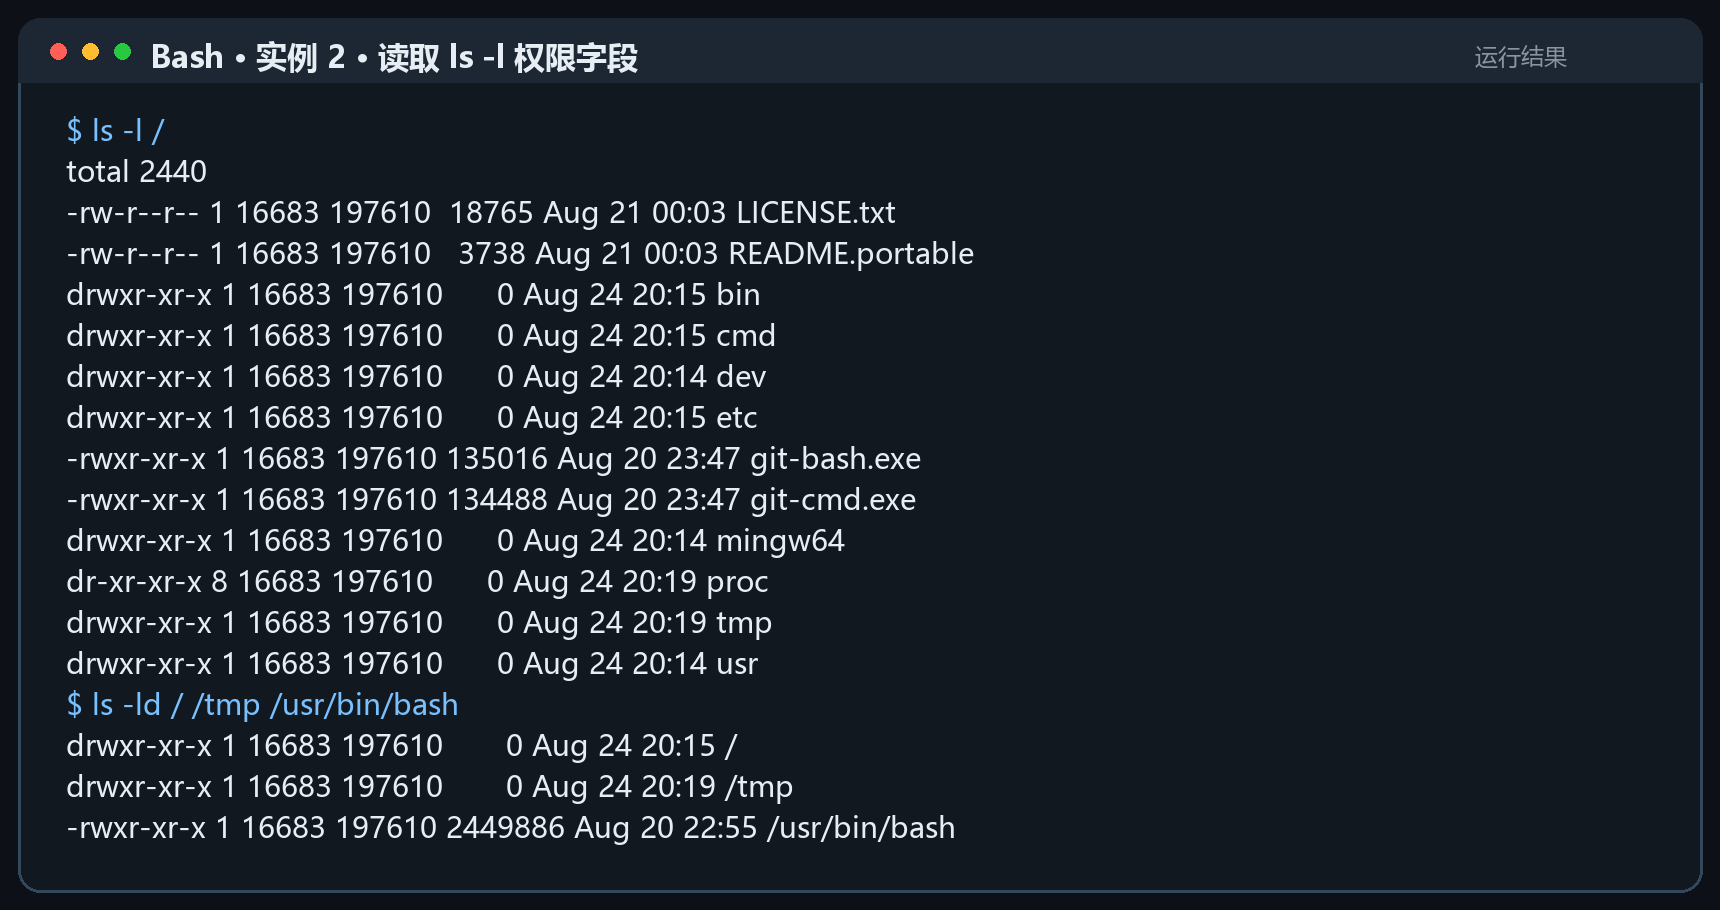
\includegraphics[width=.94\textwidth,height=.53\textheight,keepaspectratio]{assets/practice-ex02.png}
  \caption{实例 2 运行结果}
\end{figure}

\begin{summarybox}{结果说明}
\texttt{-l} 使用长格式显示文件类型、权限、链接数、所有者、组、大小和时间等信息。
每行前 10 个字符中，第 1 个字符表示文件类型；第 2--4、5--7、8--10 个字符分别表示所有者、用户组和其他用户的读、写、执行权限。
\end{summarybox}

\clearpage
\practicebanner{3}{测试 Shell glob 模式}

\subsection*{执行命令}
\begin{lstlisting}[style=shell]
mkdir -p glob-test && cd glob-test
touch a.txt b.txt c.txt file1.txt file2.txt file10.txt fileA.txt note.md
ls *.txt
ls file?.txt
ls {a,b,c}.txt
\end{lstlisting}

\begin{figure}[H]
  \centering
  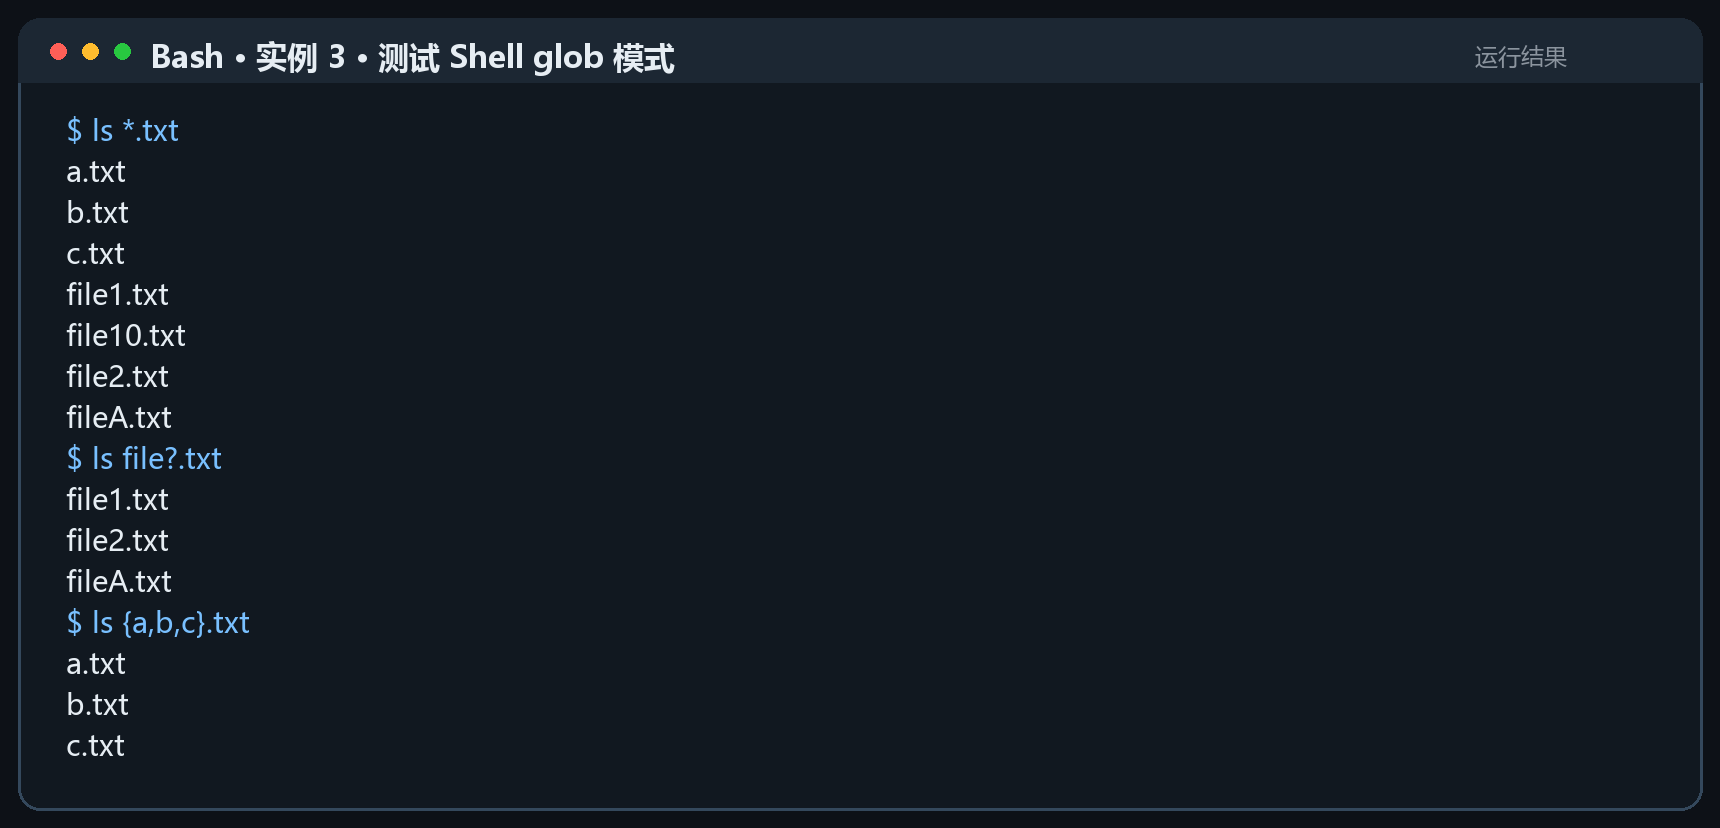
\includegraphics[width=.94\textwidth,height=.46\textheight,keepaspectratio]{assets/practice-ex03.png}
  \caption{实例 3 运行结果}
\end{figure}

\begin{summarybox}{结果说明}
\texttt{*} 匹配任意长度的字符串，\texttt{?} 恰好匹配一个字符；
\texttt{\{a,b,c\}.txt} 先展开为三个明确的文件名，因此三种模式得到不同的文件集合。
\end{summarybox}

\clearpage
\practicebanner{4}{比较三种引号}

\subsection*{执行命令}
\begin{lstlisting}[style=shell]
printf '%s\n' 'price=$5 ! \n'
printf "%s\n" "price=\$5 ! \n"
printf '%s' $'price=$5 !\nsecond line\n'
\end{lstlisting}

\begin{figure}[H]
  \centering
  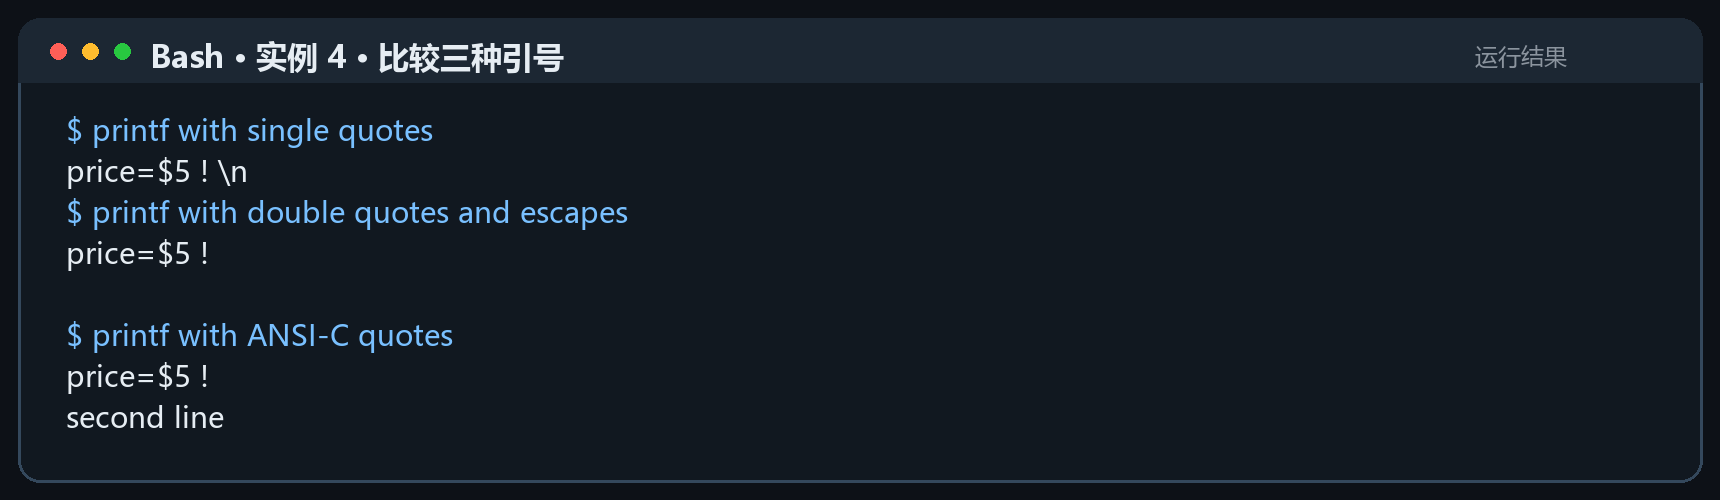
\includegraphics[width=.94\textwidth,height=.46\textheight,keepaspectratio]{assets/practice-ex04.png}
  \caption{实例 4 运行结果}
\end{figure}

\begin{summarybox}{结果说明}
单引号保留全部字符的字面值；双引号允许变量等展开，因此需要反斜杠保留美元符号；
ANSI-C 引号会解释 \texttt{\textbackslash n}，从而输出实际换行。
\end{summarybox}

\clearpage
\practicebanner{5}{重定向标准输出与错误}

\subsection*{执行命令}
\begin{lstlisting}[style=shell]
ls /nonexistent /tmp > stdout.txt 2> stderr.txt
head -n 8 stdout.txt
cat stderr.txt
ls /nonexistent /tmp > both.txt 2>&1
head -n 10 both.txt
\end{lstlisting}

\begin{figure}[H]
  \centering
  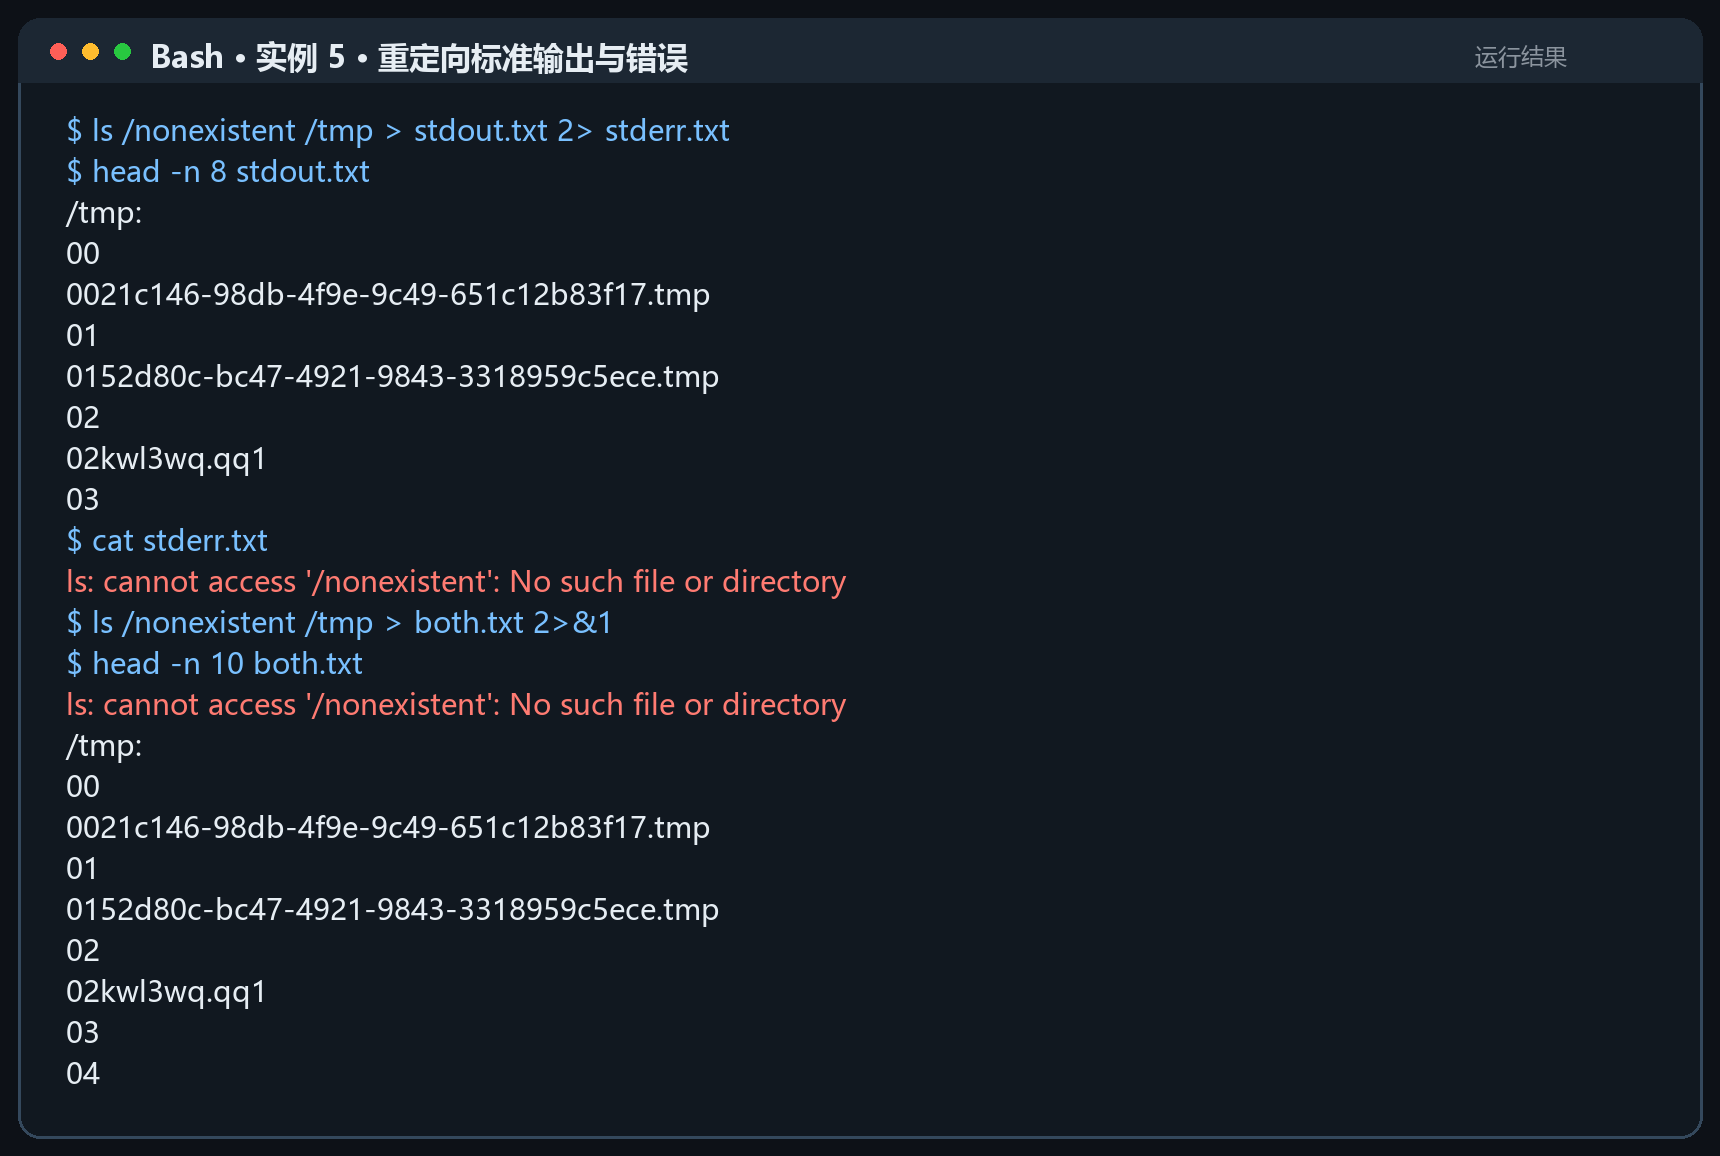
\includegraphics[width=.94\textwidth,height=.52\textheight,keepaspectratio]{assets/practice-ex05.png}
  \caption{实例 5 运行结果}
\end{figure}

\begin{summarybox}{结果说明}
\texttt{>} 将 stdout 写入 \texttt{stdout.txt}，\texttt{2>} 将 stderr 写入 \texttt{stderr.txt}；
\texttt{2>\&1} 使 stderr 指向与 stdout 相同的目标，两类信息均进入 \texttt{both.txt}。
\end{summarybox}

\clearpage
\practicebanner{6}{退出状态与条件执行}

\subsection*{执行命令}
\begin{lstlisting}[style=shell]
false; echo $?
true && echo success
false || echo fallback
target="mydir_25020007193_$$"
test -d "$target" || mkdir "$target"
ls -ld "$target"
\end{lstlisting}

\begin{figure}[H]
  \centering
  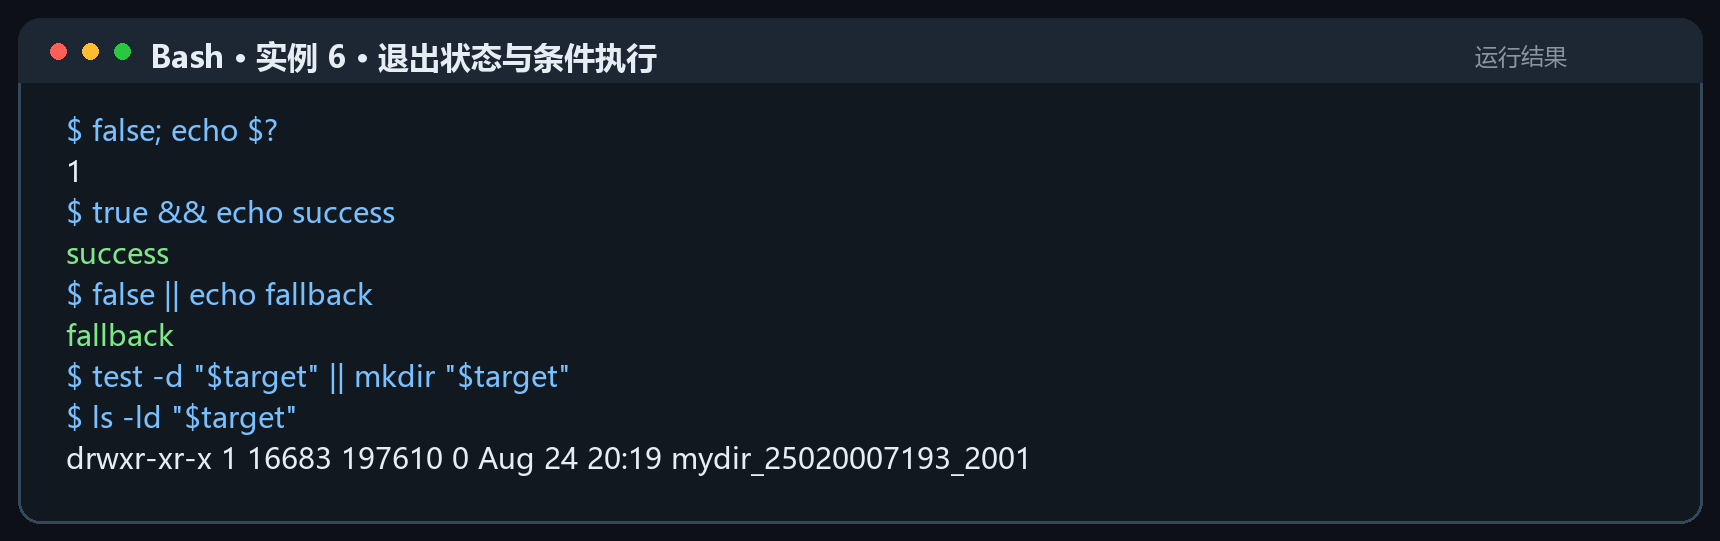
\includegraphics[width=.94\textwidth,height=.46\textheight,keepaspectratio]{assets/practice-ex06.png}
  \caption{实例 6 运行结果}
\end{figure}

\begin{summarybox}{结果说明}
\texttt{false} 的退出状态为 1；\texttt{\&\&} 仅在前一条命令成功时继续，\texttt{||} 仅在失败时继续。
目录不存在时，\texttt{test -d} 返回非零状态并触发 \texttt{mkdir}。
\end{summarybox}

\clearpage
\practicebanner{7}{验证 \texttt{cd} 是 Shell 内建命令}

\subsection*{执行命令}
\begin{lstlisting}[style=shell]
mkdir -p ex07/subdir && cd ex07
type cd
pwd
(cd subdir; pwd)
pwd
\end{lstlisting}

\begin{figure}[H]
  \centering
  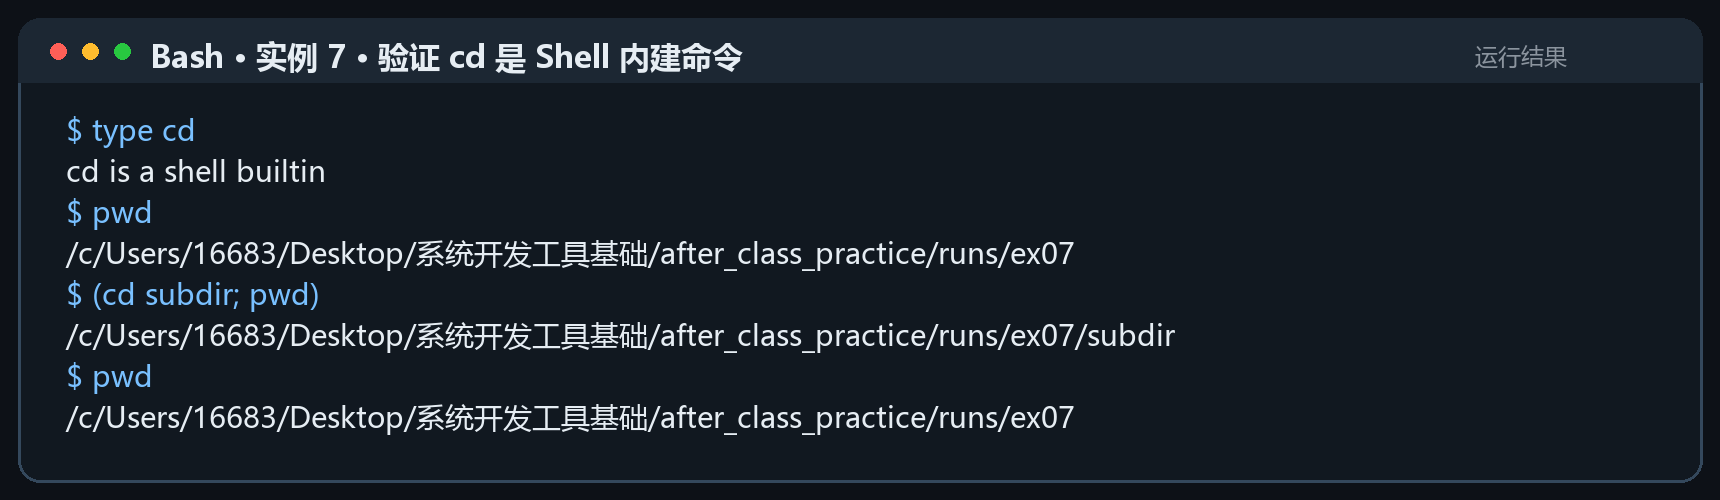
\includegraphics[width=.94\textwidth,height=.46\textheight,keepaspectratio]{assets/practice-ex07.png}
  \caption{实例 7 运行结果}
\end{figure}

\begin{summarybox}{结果说明}
\texttt{type cd} 显示 \texttt{cd} 是 Shell 内建命令。子 Shell 能改变自己的工作目录，
但结束后父 Shell 的目录保持不变；因此 \texttt{cd} 必须在当前 Shell 中直接修改目录状态。
\end{summarybox}

\clearpage
\practicebanner{8}{用脚本检查文件是否存在}

\subsection*{执行命令}
\begin{lstlisting}[style=shell]
cat > check.sh <<'EOF'
#!/usr/bin/env bash
if [ "$#" -ne 1 ]; then
    echo "Usage: $0 <file>" >&2
    exit 2
fi
if [ -f "$1" ]; then
    echo "File exists: $1"
else
    echo "File not found: $1" >&2
    exit 1
fi
EOF

printf 'sample\n' > existing.txt
bash check.sh existing.txt
bash check.sh missing.txt
echo $?
\end{lstlisting}

\begin{figure}[H]
  \centering
  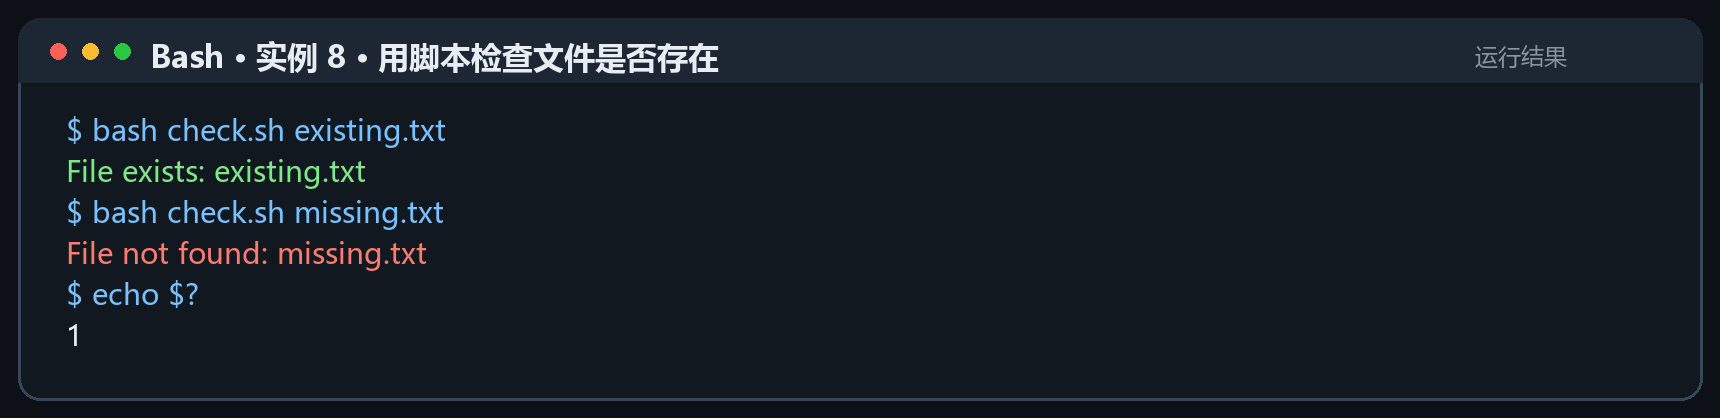
\includegraphics[width=.94\textwidth,height=.34\textheight,keepaspectratio]{assets/practice-ex08.png}
  \caption{实例 8 运行结果}
\end{figure}

\begin{summarybox}{结果说明}
脚本用 \texttt{[ -f "\$1" ]} 判断参数是否指向普通文件；存在时输出成功提示，
不存在时向 stderr 输出提示并返回退出状态 1。
\end{summarybox}

\clearpage
\practicebanner{10}{使用 \texttt{set -x} 跟踪命令}

\subsection*{执行命令}
\begin{lstlisting}[style=shell]
cat > trace.sh <<'EOF'
#!/usr/bin/env bash
set -x
name="trace-demo"
echo "hello $name"
test -f sample.txt || touch sample.txt
wc -c sample.txt
EOF

rm -f sample.txt
bash trace.sh
\end{lstlisting}

\begin{figure}[H]
  \centering
  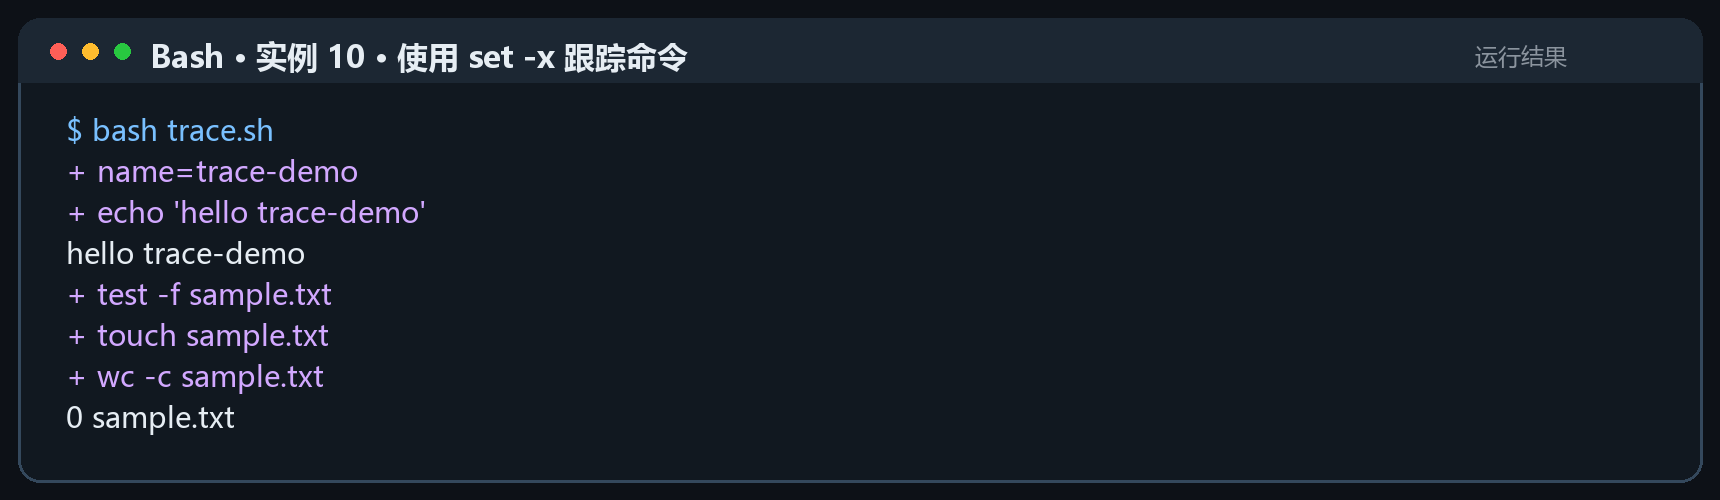
\includegraphics[width=.94\textwidth,height=.38\textheight,keepaspectratio]{assets/practice-ex10.png}
  \caption{实例 10 运行结果}
\end{figure}

\begin{summarybox}{结果说明}
\texttt{set -x} 在命令执行前输出展开后的命令，并以 \texttt{+} 标记跟踪行；
变量展开、条件判断和创建文件的执行顺序均可直接观察。
\end{summarybox}

\clearpage
\practicebanner{11}{生成带日期的备份文件名}

\subsection*{执行命令}
\begin{lstlisting}[style=shell]
printf 'week-1 notes\n' > notes.txt
cp notes.txt "notes_$(date +%Y-%m-%d).txt"
ls -l notes*.txt
cmp -s notes.txt "notes_$(date +%Y-%m-%d).txt" && echo identical
\end{lstlisting}

\begin{figure}[H]
  \centering
  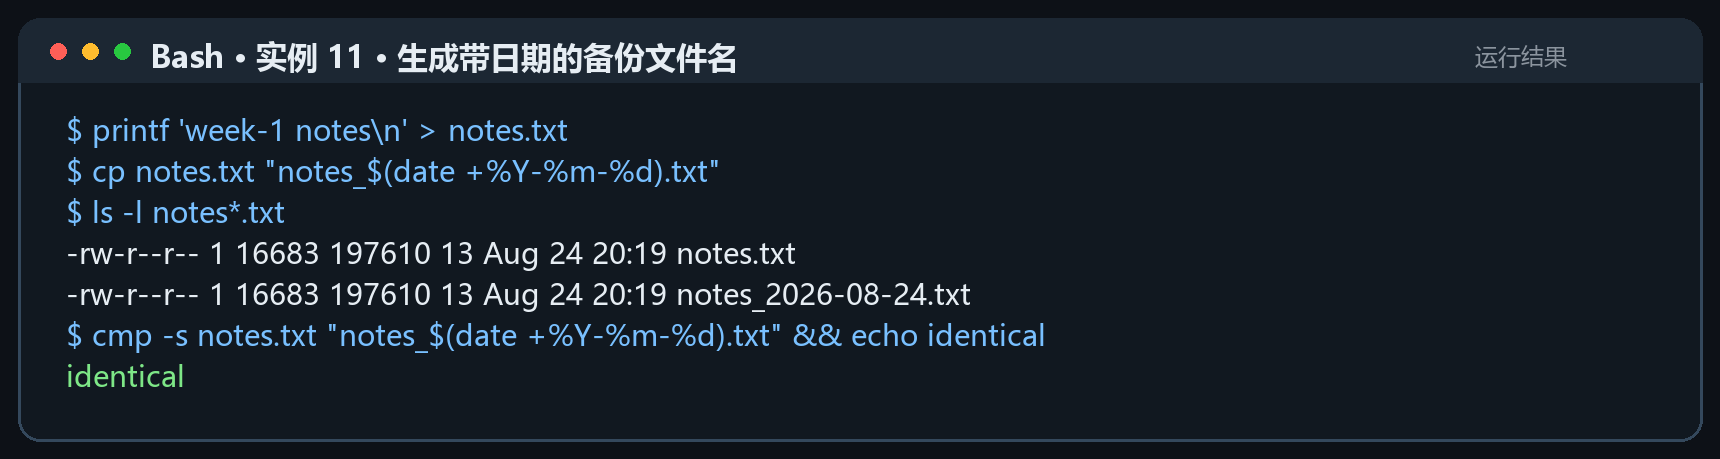
\includegraphics[width=.94\textwidth,height=.44\textheight,keepaspectratio]{assets/practice-ex11.png}
  \caption{实例 11 运行结果}
\end{figure}

\begin{summarybox}{结果说明}
命令替换 \texttt{\$(date +\%Y-\%m-\%d)} 生成当天日期并嵌入备份文件名；
\texttt{cmp -s} 验证源文件与备份内容完全一致。
\end{summarybox}

\vspace{0.7cm}
\begin{summarybox}{解题感悟}
本次实验让我更加熟悉了 Shell 文件操作、管道处理、Git 分支合并和 LaTeX 文档构建。
实践中我体会到，命令中的空格、引号和重定向符号都会直接影响结果，遇到问题应先阅读报错，
再逐步验证。通过实际执行与整理报告，我对开发工具的规范使用有了更清晰的认识。
\end{summarybox}

\vspace{0.55cm}
\begin{summarybox}{GitHub 仓库}
\centering
\url{https://github.com/FinaleQuill/system-dev-tools-foundation.git}
\end{summarybox}

\end{document}
